\documentclass[11pt,a4paper]{report}
\usepackage[textwidth=37em,vmargin=30mm]{geometry}
\usepackage{calc,xunicode,amsmath,amssymb,paralist,enumitem,tabu,booktabs,datetime2,xeCJK,xeCJKfntef,listings}
\usepackage{tocloft,fancyhdr,tcolorbox,xcolor,graphicx,eso-pic,xltxtra,xelatexemoji}

\newcommand{\envyear}[0]{2024}
\newcommand{\envdatestr}[0]{2024-10-19}
\newcommand{\envfinaldir}[0]{webdb/2024/20241019/final}

\usepackage[hidelinks]{hyperref}
\hypersetup{
    colorlinks=false,
    pdfpagemode=FullScreen,
    pdftitle={Web Digest - \envdatestr}
}

\setlength{\cftbeforechapskip}{10pt}
\renewcommand{\cftchapfont}{\rmfamily\bfseries\large\raggedright}
\setlength{\cftbeforesecskip}{2pt}
\renewcommand{\cftsecfont}{\sffamily\small\raggedright}

\setdefaultleftmargin{2em}{2em}{1em}{1em}{1em}{1em}

\usepackage{xeCJK,xeCJKfntef}
\xeCJKsetup{PunctStyle=plain,RubberPunctSkip=false,CJKglue=\strut\hskip 0pt plus 0.1em minus 0.05em,CJKecglue=\strut\hskip 0.22em plus 0.2em}
\XeTeXlinebreaklocale "zh"
\XeTeXlinebreakskip = 0pt


\setmainfont{Brygada 1918}
\setromanfont{Brygada 1918}
\setsansfont{IBM Plex Sans}
\setmonofont{JetBrains Mono NL}
\setCJKmainfont{Noto Serif CJK SC}
\setCJKromanfont{Noto Serif CJK SC}
\setCJKsansfont{Noto Sans CJK SC}
\setCJKmonofont{Noto Sans CJK SC}

\setlength{\parindent}{0pt}
\setlength{\parskip}{8pt}
\linespread{1.15}

\lstset{
	basicstyle=\ttfamily\footnotesize,
	numbersep=5pt,
	backgroundcolor=\color{black!5},
	showspaces=false,
	showstringspaces=false,
	showtabs=false,
	tabsize=2,
	captionpos=b,
	breaklines=true,
	breakatwhitespace=true,
	breakautoindent=true,
	linewidth=\textwidth
}






\newcommand{\coverpic}[2]{
    % argv: itemurl, authorname
    Cover photo by #2~~(\href{#1}{#1})
}
\newcommand{\makeheader}[0]{
    \begin{titlepage}
        % \newgeometry{hmargin=15mm,tmargin=21mm,bmargin=12mm}
        \begin{center}
            
            \rmfamily\scshape
            \fontspec{BaskervilleF}
            \fontspec{Old Standard}
            \fontsize{59pt}{70pt}\selectfont
            WEB\hfill DIGEST
            
            \vfill
            % \vskip 30pt
            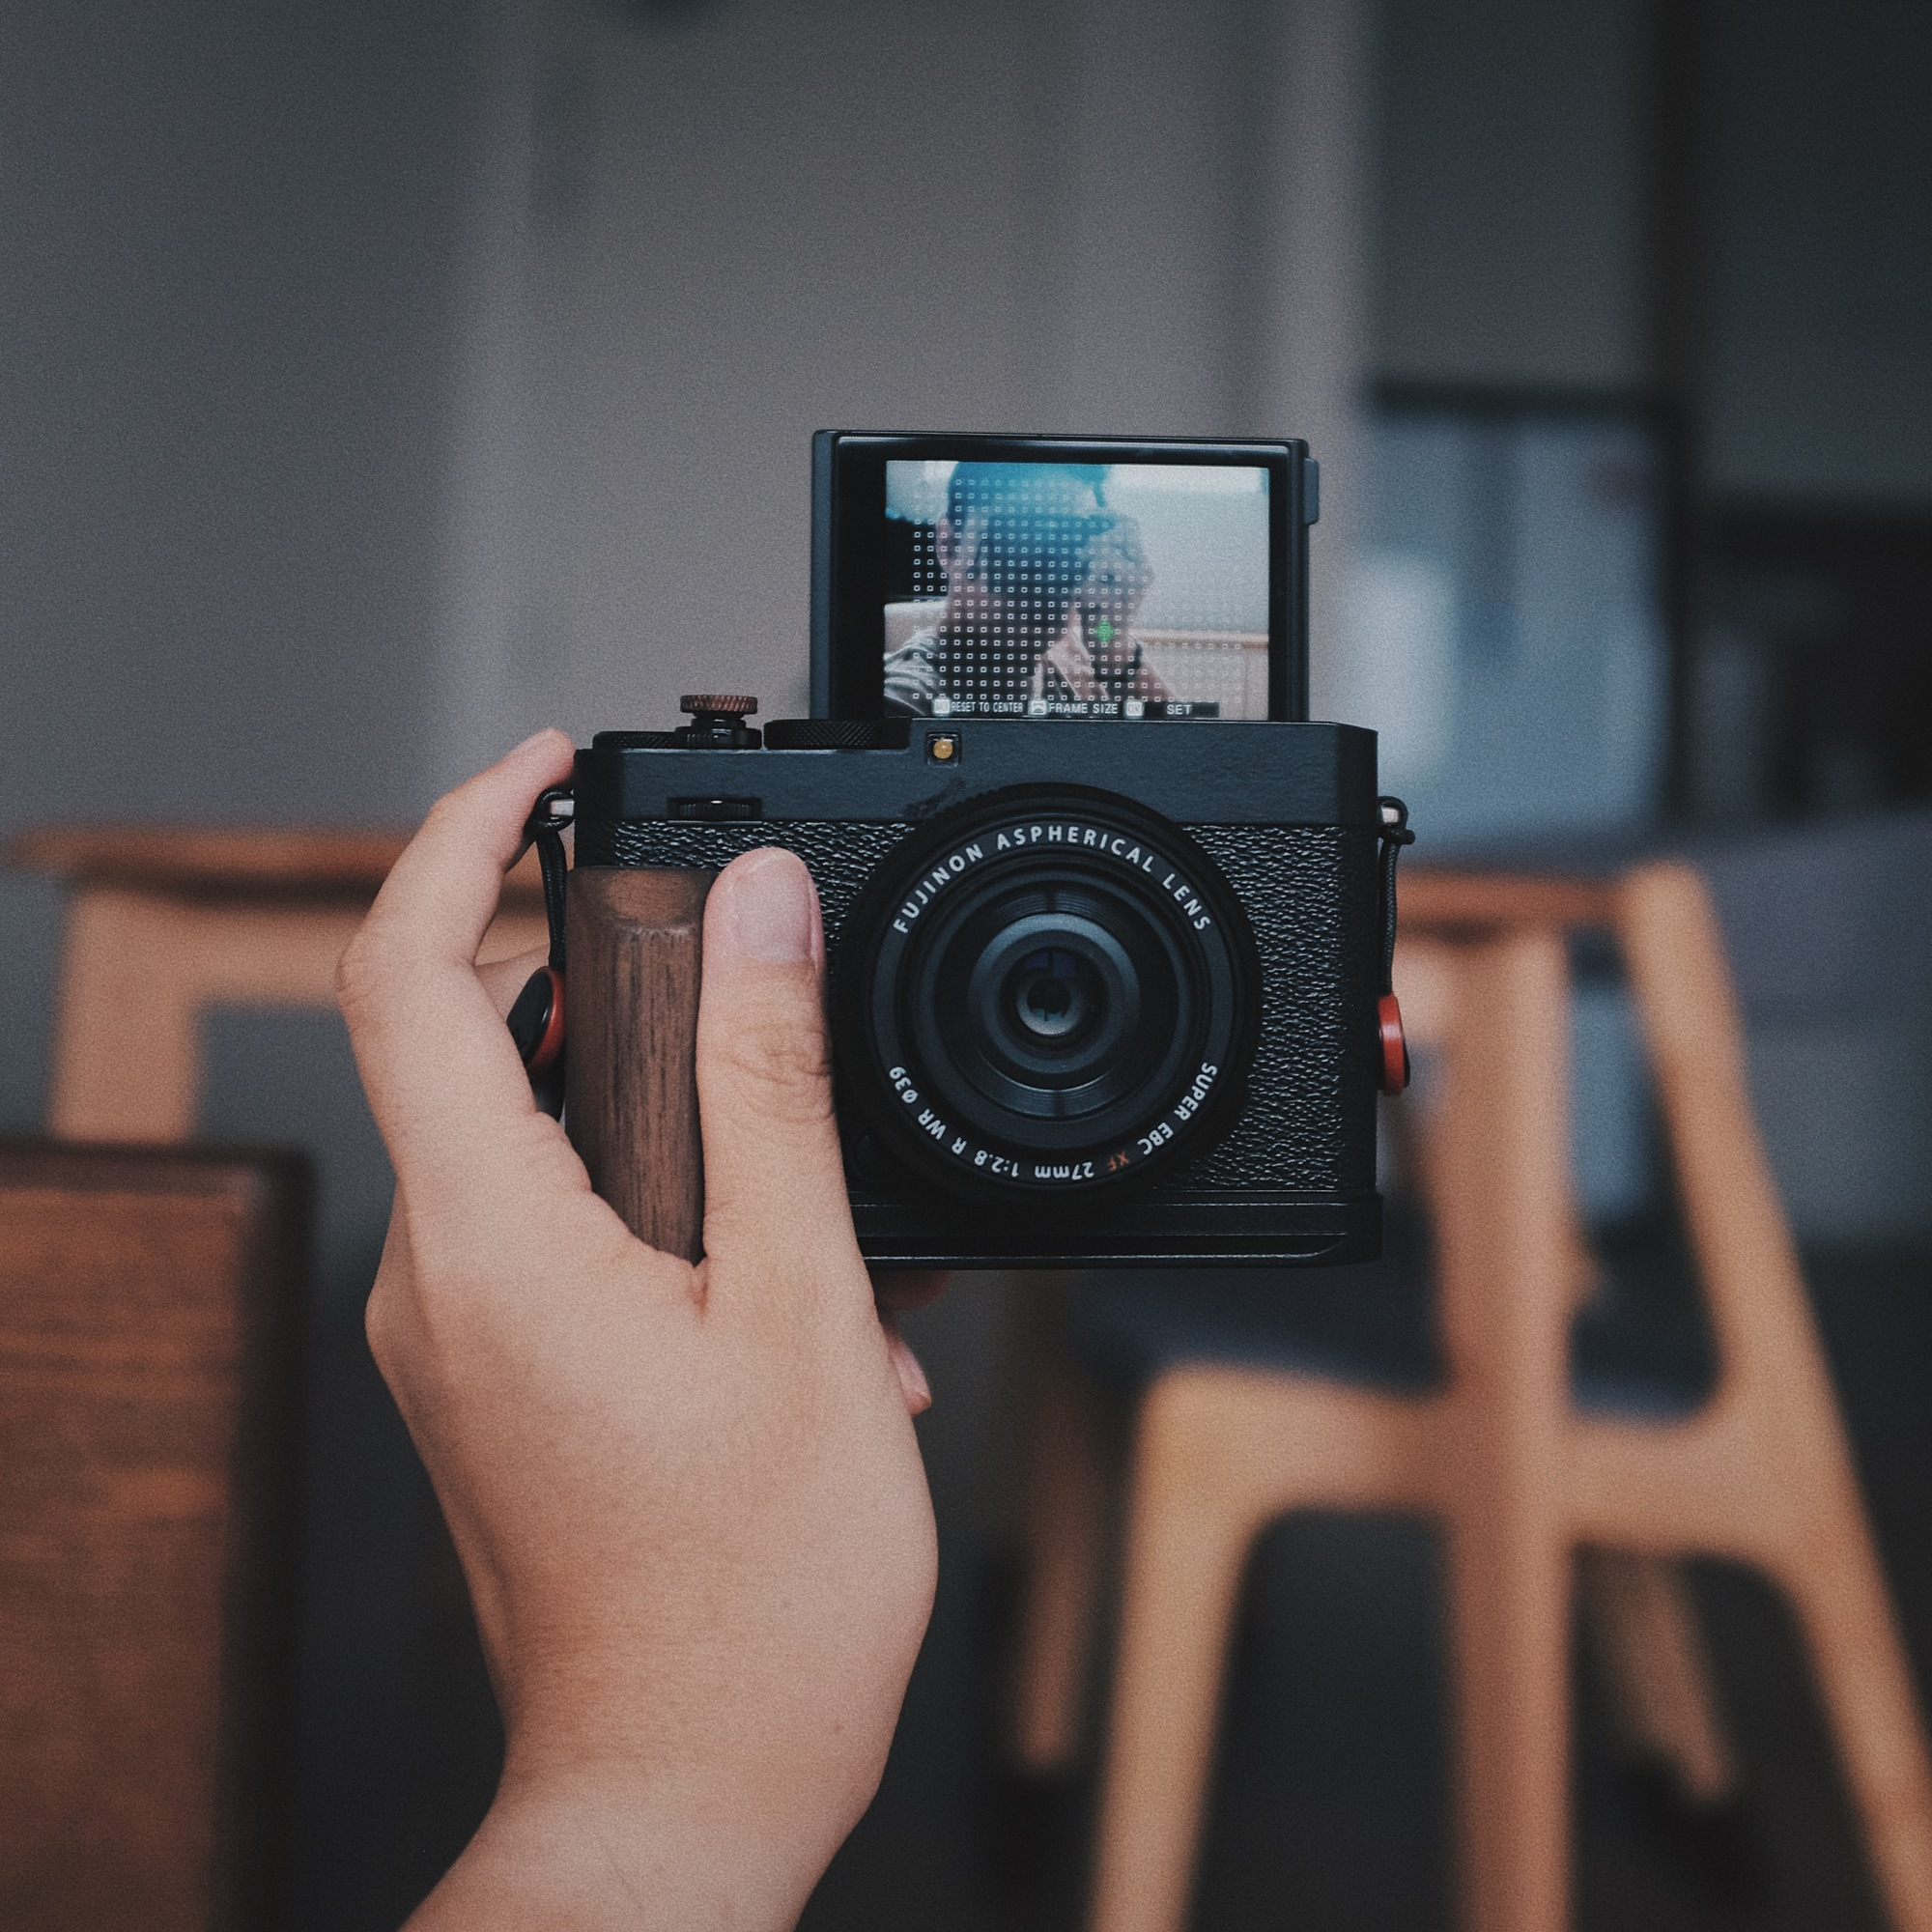
\includegraphics[width=\linewidth]{\envfinaldir/coverpic-prod.jpg}\par
            % \vskip 30pt
            \vfill

            \normalsize\rmfamily\scshape
            \copyright{} The Web Digest Project \hfill\large \envdatestr
        \end{center}
    \end{titlepage}
    % \restoregeometry
}
\newcommand{\simplehref}[1]{%
    \textcolor{blue!80!green}{\href{#1}{#1}}%
}
\renewcommand{\contentsname}{\center\Huge\sffamily\bfseries Contents\par\vskip 20pt}
\newcounter{ipartcounter}
\setcounter{ipartcounter}{0}
\newcommand{\ipart}[1]{
    % \vskip 20pt
    \clearpage
    \stepcounter{ipartcounter}
    \phantomsection
    \addcontentsline{toc}{chapter}{#1}
    % \begin{center}
    %     \Huge
    %     \sffamily\bfseries
    %     #1
    % \end{center}
    % \vskip 20pt plus 7pt
}
\newcounter{ichaptercounter}
\setcounter{ichaptercounter}{0}
\newcommand{\ichapter}[1]{
    % \vskip 20pt
    \clearpage
    \stepcounter{ichaptercounter}
    \phantomsection
    \addcontentsline{toc}{section}{\numberline{\arabic{ichaptercounter}}#1}
    \begin{center}
        \Huge
        \sffamily\bfseries
        #1
    \end{center}
    \vskip 20pt plus 7pt
}
\newcommand{\entrytitlefont}[1]{\subsection*{\raggedright\Large\sffamily\bfseries#1}}
\newcommand{\entryitemGeneric}[2]{
    % argv: title, url
    \parbox{\linewidth}{
        \entrytitlefont{#1}\par\vskip 5pt
        \footnotesize\ttfamily\mdseries
        \simplehref{#2}
    }\vskip 11pt plus 11pt minus 1pt
}
\newcommand{\entryitemGithub}[3]{
    % argv: title, url, desc
    \parbox{\linewidth}{
        \entrytitlefont{#1}\par\vskip 5pt
        \footnotesize\ttfamily\mdseries
        \simplehref{#2}\par\vskip 5pt
        \small\rmfamily\mdseries#3
    }\vskip 11pt plus 11pt minus 1pt
}
\newcommand{\entryitemAp}[3]{
    % argv: title, url, desc
    \parbox{\linewidth}{
        \entrytitlefont{#1}\par\vskip 5pt
        \footnotesize\ttfamily\mdseries
        \simplehref{#2}\par\vskip 5pt
        \small\rmfamily\mdseries#3
    }\vskip 11pt plus 11pt minus 1pt
}
\newcommand{\entryitemHackernews}[3]{
    % argv: title, hnurl, rawurl
    % \parbox{\linewidth}{
    %     \entrytitlefont{#1}\par\vskip 5pt
    %     \footnotesize\ttfamily\mdseries
    %     \simplehref{#3}\par
    %     \textcolor{black!50}{\href{#2}{#2}}
    % }\vskip 11pt plus 11pt minus 1pt
    \begin{minipage}{\linewidth}
            \entrytitlefont{#1}\par\vskip 5pt
            \footnotesize\ttfamily\mdseries
            \simplehref{#3}\par
            \textcolor{black!50}{\href{#2}{#2}}
    \end{minipage}\par\vskip 11pt plus 11pt minus 1pt
}







\begin{document}

\makeheader

\tableofcontents\clearpage




\ipart{Developers}
\ichapter{Hacker News}
\entryitemTwoLinks{The feds are coming for John Deere over the right to repair}{https://news.ycombinator.com/item?id=41880981}{https://gizmodo.com/the-feds-are-coming-for-john-deere-over-the-right-to-repair-2000513521}

\entryitemTwoLinks{Subvert – Collectively owned music marketplace}{https://news.ycombinator.com/item?id=41880829}{https://subvert.fm/}

\entryitemTwoLinks{Show HN: Go Plan9 Memo}{https://news.ycombinator.com/item?id=41879854}{https://pehringer.info/go\_plan9\_memo.html}

\entryitemTwoLinks{Running an open source app: Usage, costs and community donations}{https://news.ycombinator.com/item?id=41879845}{https://spliit.app/blog/spliit-by-the-stats-usage-costs-donations}

\entryitemTwoLinks{Code that helped end Apartheid}{https://news.ycombinator.com/item?id=41879072}{https://www.wired.com/story/plaintext-you-can-now-see-the-code-that-ended-apartheid/}

\entryitemTwoLinks{Apple Passwords' generated strong password format}{https://news.ycombinator.com/item?id=41878290}{https://rmondello.com/2024/10/07/apple-passwords-generated-strong-password-format/}

\entryitemTwoLinks{Microsoft and OpenAI's close partnership shows signs of fraying}{https://news.ycombinator.com/item?id=41878281}{https://www.nytimes.com/2024/10/17/technology/microsoft-openai-partnership-deal.html}

\entryitemTwoLinks{Impact of early life adversity on reward processing in young adults (2014)}{https://news.ycombinator.com/item?id=41878167}{https://journals.plos.org/plosone/article?id=10.1371/journal.pone.0104185}

\entryitemTwoLinks{Net 9.0 LINQ Performance Improvements}{https://news.ycombinator.com/item?id=41878095}{https://blog.ndepend.com/net-9-0-linq-performance-improvements/}

\entryitemTwoLinks{Microsoft BitNet: inference framework for 1-bit LLMs}{https://news.ycombinator.com/item?id=41877609}{https://github.com/microsoft/BitNet}

\entryitemTwoLinks{Secret 3D scans in the French Supreme Court}{https://news.ycombinator.com/item?id=41877513}{https://cosmowenman.substack.com/p/secret-3d-scans-in-the-french-supreme}

\entryitemTwoLinks{Life is not a story}{https://news.ycombinator.com/item?id=41876979}{https://psyche.co/ideas/your-life-is-not-a-story-why-narrative-thinking-holds-you-back}

\entryitemTwoLinks{Factorio – Visualizing construction material dependencies}{https://news.ycombinator.com/item?id=41876821}{https://community.wolfram.com/groups/-/m/t/1793319}

\entryitemTwoLinks{Using static websites for tiny archives}{https://news.ycombinator.com/item?id=41876750}{https://alexwlchan.net/2024/static-websites/}

\entryitemTwoLinks{What is theoretical computer science?}{https://news.ycombinator.com/item?id=41876723}{https://cacm.acm.org/opinion/what-is-theoretical-computer-science/}

\entryitemTwoLinks{Kennedy, Merkley introduce bill to end TSA facial recognition (2023)}{https://news.ycombinator.com/item?id=41876071}{https://www.kennedy.senate.gov/public/2023/11/kennedy-merkley-introduce-bill-to-end-involuntary-facial-recognition-screenings-protect-americans-privacy}

\entryitemTwoLinks{Smart pointers for the kernel}{https://news.ycombinator.com/item?id=41875792}{https://lwn.net/Articles/992055/}

\entryitemTwoLinks{SOFA - Start Often Finish rArely}{https://news.ycombinator.com/item?id=41875108}{https://tilde.town/~dozens/sofa/}

\entryitemTwoLinks{C++ proposal: There are exactly 8 bits in a byte}{https://news.ycombinator.com/item?id=41874394}{https://www.open-std.org/jtc1/sc22/wg21/docs/papers/2024/p3477r0.html}

\entryitemTwoLinks{The Fifth Generation Project in Japan (1992)}{https://news.ycombinator.com/item?id=41874275}{https://www.sjsu.edu/faculty/watkins/5thgen.htm}\ichapter{Phoronix}
\entryitemGeneric{\hskip 0pt{}Intel Working On Coreboot Support For Xeon 6 Platforms}{https://www.phoronix.com/news/Intel-Xeon-6-Coreboot-Effort}

\entryitemGeneric{\hskip 0pt{}Wine 9.20 Released With WineDbg Now Using Capstone Disassembler}{https://www.phoronix.com/news/Wine-9.20-Released}

\entryitemGeneric{\hskip 0pt{}Ubuntu Considers Replacing initramfs-tools WIth Dracut}{https://www.phoronix.com/news/Ubuntu-Considers-Dracut-Initrd}

\entryitemGeneric{\hskip 0pt{}Linux 6.13 Poised To Land Prep Patches Working Toward Proxy Execution}{https://www.phoronix.com/news/Linux-6.13-Prep-For-Proxy-Exec}

\entryitemGeneric{\hskip 0pt{}Linux Fixes Indirect Branch Predictor Barrier "IBPB" Handling For Older AMD CPUs}{https://www.phoronix.com/news/Linux-AMD-Fixes-IBPB-Older-CPUs}

\entryitemGeneric{\hskip 0pt{}Laptop Vendor MALIBAL Suggests Not Supporting Coreboot}{https://www.phoronix.com/news/Malibal-Suggests-No-Coreboot}

\entryitemGeneric{\hskip 0pt{}AMD ROCm Looks Like It Will Finally Be Supporting OpenCL 3.0 Soon}{https://www.phoronix.com/news/AMD-ROCm-OpenCL-3.0-Soon}

\entryitemGeneric{\hskip 0pt{}Ubuntu Snaps Up Intel's NPU User-Space Software So It's Easier To Accelerate AI}{https://www.phoronix.com/news/Ubuntu-Snaps-Intel-NPU-Driver}

\entryitemGeneric{\hskip 0pt{}Valve Contributes OpenVR Video Driver To SDL}{https://www.phoronix.com/news/SDL-OpenVR-Video-Driver}


\ipart{Developers~~~~(zh-Hans)}
\ichapter{Solidot}
\entryitemGeneric{\hskip 0pt{}亚马逊高管告诉员工如果不喜欢强制重返办公室政策他们可以辞职}{https://www.solidot.org/story?sid=79534}

\entryitemGeneric{\hskip 0pt{}人类的嗅觉反应十分迅速}{https://www.solidot.org/story?sid=79533}

\entryitemGeneric{\hskip 0pt{}OpenAI 和微软的紧密关系出现裂缝}{https://www.solidot.org/story?sid=79532}

\entryitemGeneric{\hskip 0pt{}Gliese 229 B 被发现是一对棕矮星}{https://www.solidot.org/story?sid=79531}

\entryitemGeneric{\hskip 0pt{}高中生因使用 AI 受罚,其父母随后起诉教师和校长}{https://www.solidot.org/story?sid=79530}

\entryitemGeneric{\hskip 0pt{}新疗法能消除 2 型糖尿病患者对胰岛素的需求}{https://www.solidot.org/story?sid=79529}

\entryitemGeneric{\hskip 0pt{}欧盟考虑将马斯克其他公司的收入纳入 X 的潜在罚款计算内}{https://www.solidot.org/story?sid=79528}

\entryitemGeneric{\hskip 0pt{}NASA 冻结波音 Starliner 任务}{https://www.solidot.org/story?sid=79527}

\entryitemGeneric{\hskip 0pt{}香港诈骗集团用 AI 深度伪造欺骗受害者}{https://www.solidot.org/story?sid=79526}

\entryitemGeneric{\hskip 0pt{}Meta 解雇了 20 多名用餐券购买家庭用品的员工}{https://www.solidot.org/story?sid=79525}

\entryitemGeneric{\hskip 0pt{}养殖鱼比野生捕捞更不可持续}{https://www.solidot.org/story?sid=79524}

\entryitemGeneric{\hskip 0pt{}Telegram 有数百万用户利用 AI 制作深度伪造色情}{https://www.solidot.org/story?sid=79523}

\entryitemGeneric{\hskip 0pt{}美国起诉了两名 Anonymous Sudan 成员}{https://www.solidot.org/story?sid=79522}

\entryitemGeneric{\hskip 0pt{}保持互联网运行的深海紧急任务}{https://www.solidot.org/story?sid=79521}

\entryitemGeneric{\hskip 0pt{}Matt Mullenweg 的报复行动冲击 WordPress 社区}{https://www.solidot.org/story?sid=79520}

\entryitemGeneric{\hskip 0pt{}哈勃发现木星大红斑大小会变化}{https://www.solidot.org/story?sid=79519}

\entryitemGeneric{\hskip 0pt{}官方机构指责英特尔产品存在网络安全问题}{https://www.solidot.org/story?sid=79518}

\entryitemGeneric{\hskip 0pt{}Twitter/X 将使用用户帖子训练 AI,这一次用户无法退出}{https://www.solidot.org/story?sid=79517}

\entryitemGeneric{\hskip 0pt{}腾讯微信使用的 MMTLS 加密协议存在安全弱点}{https://www.solidot.org/story?sid=79516}

\entryitemGeneric{\hskip 0pt{}高收入的低稳定性}{https://www.solidot.org/story?sid=79515}\ichapter{V2EX}
\entryitemGeneric{\hskip 0pt{}[问与答] 国标插座是工业国里最烂的插座标准么?}{https://www.v2ex.com/t/1081654}

\entryitemGeneric{\hskip 0pt{}[酷工作] 印第安纳大学 Luddy 信息、计算与工程学院 Dr. Yan Zhuang 课题组 2025 年全奖博士生招募}{https://www.v2ex.com/t/1081653}

\entryitemGeneric{\hskip 0pt{}[分享创造] 画布和涂鸦文字核心的社交产品创意。}{https://www.v2ex.com/t/1081652}

\entryitemGeneric{\hskip 0pt{}[程序员] 鸿蒙 next 的 app,积累的屎山都没了}{https://www.v2ex.com/t/1081651}

\entryitemGeneric{\hskip 0pt{}[分享发现] 京东金融有项目触发巨额赎回了}{https://www.v2ex.com/t/1081650}

\entryitemGeneric{\hskip 0pt{}[iPhone] 求现在 24 年 10 月注册美区 apple id 的办法?}{https://www.v2ex.com/t/1081649}

\entryitemGeneric{\hskip 0pt{}[分享发现] 原来 AI 也会玩恶作剧啊....}{https://www.v2ex.com/t/1081648}

\entryitemGeneric{\hskip 0pt{}[macOS] 求外置移动硬盘推荐}{https://www.v2ex.com/t/1081647}

\entryitemGeneric{\hskip 0pt{}[程序员] 记录对 pm2 的操作误解}{https://www.v2ex.com/t/1081646}

\entryitemGeneric{\hskip 0pt{}[Apple] 苹果审核巨慢}{https://www.v2ex.com/t/1081644}

\entryitemGeneric{\hskip 0pt{}[Kindle] 新 kindle 太好看了,翻页操作速度也接近手机了}{https://www.v2ex.com/t/1081643}

\entryitemGeneric{\hskip 0pt{}[问与答] 搜狗输入法通过 Windows 通知来推送广告,而且关闭通知的按钮是灰色的}{https://www.v2ex.com/t/1081642}

\entryitemGeneric{\hskip 0pt{}[优惠信息] pockethost.io 永久版开售}{https://www.v2ex.com/t/1081641}

\entryitemGeneric{\hskip 0pt{}[VPS] 出 2 个闲置的 VPS,厂商 colocrossing, 25 年 3 月 30 到七}{https://www.v2ex.com/t/1081640}

\entryitemGeneric{\hskip 0pt{}[NAS] ipv6 访问慢}{https://www.v2ex.com/t/1081639}

\entryitemGeneric{\hskip 0pt{}[问与答] SOCKS5 转成 L2tp}{https://www.v2ex.com/t/1081638}

\entryitemGeneric{\hskip 0pt{}[Windows] 如何禁止 Windows11 ,自动安全扫描后,弹出的提示}{https://www.v2ex.com/t/1081637}

\entryitemGeneric{\hskip 0pt{}[问与答] [成都-技术支持转行嵌入式经历帖-02] 在迷雾中勇敢地摸索中前行}{https://www.v2ex.com/t/1081636}

\entryitemGeneric{\hskip 0pt{}[宽带症候群] 珠江宽频改公网后晚上限制 TCP 连接数 1000}{https://www.v2ex.com/t/1081635}

\entryitemGeneric{\hskip 0pt{}[酷工作] [远程][兼职/全职] 本地 AI 搜索引擎 Gety 招聘啦}{https://www.v2ex.com/t/1081634}

\entryitemGeneric{\hskip 0pt{}[API] 有哪些开源程序可以快速构建 API 服务}{https://www.v2ex.com/t/1081633}

\entryitemGeneric{\hskip 0pt{}[问与答] 推荐一个降噪好+没有电量低提示的 tws 耳机}{https://www.v2ex.com/t/1081631}

\entryitemGeneric{\hskip 0pt{}[OpenAI] 请给个建议,招个人写提示词.该怎么操作才合理呢?}{https://www.v2ex.com/t/1081629}

\entryitemGeneric{\hskip 0pt{}[生活] 近况:找工作\&生活\&租房都不顺(朋友们帮忙判断下租房的事是我的问题?)}{https://www.v2ex.com/t/1081628}

\entryitemGeneric{\hskip 0pt{}[云计算] 阿里云 HK 的 DNS 解析 google 地址不正确}{https://www.v2ex.com/t/1081627}

\entryitemGeneric{\hskip 0pt{}[iPhone] 大家的 iPhone14p 电池健康度还有多少?}{https://www.v2ex.com/t/1081626}

\entryitemGeneric{\hskip 0pt{}[问与答] 请教一下搞电商的朋友, amazon 被独立站抄袭并恶意投诉,有没有办法证明对方的网页创建时间晚于我们的?}{https://www.v2ex.com/t/1081624}

\entryitemGeneric{\hskip 0pt{}[Android] 这个优道省电助手怎么删除}{https://www.v2ex.com/t/1081623}

\entryitemGeneric{\hskip 0pt{}[问与答] 求推荐汽车行车记录仪}{https://www.v2ex.com/t/1081622}

\entryitemGeneric{\hskip 0pt{}[分享创造] 做了一个浏览器 app,可以为大家免费推广产品}{https://www.v2ex.com/t/1081621}

\entryitemGeneric{\hskip 0pt{}[问与答] 最近汽水音乐增加了开屏广告,开通 SVIP 后免广告(普通 VIP 不免),大家怎么看?}{https://www.v2ex.com/t/1081620}

\entryitemGeneric{\hskip 0pt{}[投资] 回馈 v 站,送给新韭菜}{https://www.v2ex.com/t/1081619}

\entryitemGeneric{\hskip 0pt{}[Android] 安卓系统容易中病毒吗?}{https://www.v2ex.com/t/1081618}

\entryitemGeneric{\hskip 0pt{}[问与答] 关于 2FA 码的一个小问题}{https://www.v2ex.com/t/1081615}

\entryitemGeneric{\hskip 0pt{}[C++] C++ 新手想问下关于 Linux 下如何实现类似 Windows 的 Pause 功能的问题}{https://www.v2ex.com/t/1081614}

\entryitemGeneric{\hskip 0pt{}[宽带症候群] 爱快老是掉 v6 的 pd 前缀是啥情况?}{https://www.v2ex.com/t/1081611}

\entryitemGeneric{\hskip 0pt{}[问与答] po 于上班喝咖啡,求推荐胶囊咖啡机}{https://www.v2ex.com/t/1081610}

\entryitemGeneric{\hskip 0pt{}[程序员] 字节跳动有个实习生往商业化整个 gpu 集群里注入病毒,导致一个月的训练结果不可用}{https://www.v2ex.com/t/1081609}

\entryitemGeneric{\hskip 0pt{}[全球工单系统] 京东以旧换新活动的离谱规定}{https://www.v2ex.com/t/1081608}

\entryitemGeneric{\hskip 0pt{}[奇思妙想] 假如有这么个政策,是不是可以解决当下的问题}{https://www.v2ex.com/t/1081607}

\entryitemGeneric{\hskip 0pt{}[程序员] 同样功能界面,是不是 H5 开发比 iOS 原生开发速度快}{https://www.v2ex.com/t/1081606}

\entryitemGeneric{\hskip 0pt{}[问与答] ChatGPT 的 stt 是用的 whisper 吗? 感觉比所有其他的语音输入都要强}{https://www.v2ex.com/t/1081605}

\entryitemGeneric{\hskip 0pt{}[问与答] 2024 有什么能用的网络电话,国内环境使用,不会奇怪的号码}{https://www.v2ex.com/t/1081604}

\entryitemGeneric{\hskip 0pt{}[职场话题] 记一次杭州银行面试,踩雷}{https://www.v2ex.com/t/1081603}

\entryitemGeneric{\hskip 0pt{}[酷工作] 上海张江国企: Java 架构师, 40-50W,希望可以快速到岗}{https://www.v2ex.com/t/1081601}

\entryitemGeneric{\hskip 0pt{}[问与答] 天天坐在电脑前,到底该选一个什么样的椅子?}{https://www.v2ex.com/t/1081600}

\entryitemGeneric{\hskip 0pt{}[问与答] 想换个手机求推荐}{https://www.v2ex.com/t/1081598}

\entryitemGeneric{\hskip 0pt{}[ WATCH] 随手表带的线不能充苹果耳机了?}{https://www.v2ex.com/t/1081597}

\entryitemGeneric{\hskip 0pt{}[分享发现] V 站好像很多朋友不懂硬件,这不双十一了,给大家分享一下我的装机配置单,主打超高性价比。}{https://www.v2ex.com/t/1081595}

\entryitemGeneric{\hskip 0pt{}[买买买] 双十一求推荐空调}{https://www.v2ex.com/t/1081594}


\ipart{Generic News}
\ichapter{AP News}
\entryitemWithDescription{\hskip 0pt{}Pumpkin weighing 2,471 pounds wins California contest}{https://apnews.com/article/71cc6201bb732f057261d452bdf97ba5}{}\ichapter{Reuters}
\entryitemWithDescription{\hskip 0pt{}Explainer: How Cuba's electrical grid collapsed and what comes next}{https://www.reuters.com/world/americas/how-cubas-electrical-grid-collapsed-what-comes-next-2024-10-18/}{Cuba\textquotesingle s national grid collapsed on Friday, leaving the entire population of 10 million people without electricity and underscoring the precarious state of the Communist-run country\textquotesingle s infrastructure and...}

\entryitemWithDescription{\hskip 0pt{}Biden visit to Amazon rainforest planned in November, sources say}{https://www.reuters.com/world/biden-visit-amazon-rainforest-planned-november-sources-say-2024-10-18/}{U.S. President Joe Biden is expected to visit the Amazon rainforest and meet Brazilian President Luiz Inacio Lula da Silva before they attend the G20 summit in Rio de Janeiro in November, sources familiar with the negotiations told...}

\entryitemWithDescription{\hskip 0pt{}Trump says he would impose tariffs on China if China went into Taiwan}{https://www.reuters.com/world/trump-says-he-would-impose-tariffs-china-if-china-went-into-taiwan-2024-10-18/}{Republican presidential candidate Donald Trump said he would impose additional tariffs on China if China were to "go into Taiwan," the Wall Street Journal...}

\entryitemWithDescription{\hskip 0pt{}Gunmen attack Sinaloan media outlet amid intra-cartel war}{https://www.reuters.com/world/americas/gunmen-attack-sinaloan-media-outlet-amid-intra-cartel-war-2024-10-18/}{Gunmen sprayed with bullets the office building and several cars of respected Sinaloan media outlet El Debate on Friday, the news organization said, amid a bloody war between the two biggest factions of the Sinaloa...}

\entryitemWithDescription{\hskip 0pt{}Exclusive: Pro-Trump group funded by Musk struggles with outreach targets, inflation of doorknocking figures}{https://www.reuters.com/world/us/pro-trump-group-funded-by-musk-struggles-with-outreach-targets-inflation-2024-10-18/}{The political action committee funded by billionaire Elon Musk to help re-elect former U.S. President Donald Trump is struggling in some swing states to meet doorknocking goals and is investigating claims that some canvassers lied about...}

\entryitemWithDescription{\hskip 0pt{}Colombian coca leaf farming hit two-decade high in 2023, UN says}{https://www.reuters.com/world/americas/colombian-coca-leaf-farming-hit-two-decade-high-2023-un-says-2024-10-18/}{Colombian land dedicated to the cultivation of coca leaves, a raw ingredient for cocaine, jumped 10\% last year to reach the largest area in over two decades, a report by the United Nations Office on Drugs and Crime (UNODC) found on...}

\entryitemWithDescription{\hskip 0pt{}Some Lebanese Americans endorse Harris, expect more Lebanon support}{https://www.reuters.com/world/us/some-lebanese-americans-endorse-harris-expect-more-lebanon-support-2024-10-18/}{Some prominent Lebanese Americans on Friday endorsed Democrat Kamala Harris for president, saying in a letter that the U.S. had been "unrelenting" in its support for Lebanon under the Biden administration and they expect additional...}

\entryitemWithDescription{\hskip 0pt{}North Korea says it recovered crashed South Korean military drone, KCNA says}{https://www.reuters.com/world/asia-pacific/north-korea-says-it-recovered-crashed-south-korean-military-drone-kcna-2024-10-18/}{North Korea said it had discovered the remains of a crashed South Korean military drone, state media KCNA reported on...}

\entryitemWithDescription{\hskip 0pt{}Yemen's Houthis say they targeted ship in Arabian sea with drones}{https://www.reuters.com/world/middle-east/yemens-houthis-say-they-targeted-ship-arabian-sea-with-drones-2024-10-18/}{Yemen\textquotesingle s Houthis said on Friday they targeted a ship, which they identified as Megalopolis, in the Arabian Sea with drones, without specifying a...}

\entryitemWithDescription{\hskip 0pt{}Tunisia sentences prominent opponent Noureddine Bhiri to 10 years in prison}{https://www.reuters.com/world/africa/tunisia-sentences-prominent-opponent-noureddine-bhiri-10-years-prison-2024-10-18/}{Tunisian court sentenced on Friday the prominent official in Ennahda opposition party Noureddine Bhiri to 10 years in prison, on charges of attacking state security and inciting Tunisians against each other, a lawyer told...}

\entryitemWithDescription{\hskip 0pt{}Russia, Ukraine each bring home 95 prisoners of war in swap brokered by UAE}{https://www.reuters.com/world/europe/russia-ukraine-each-swap-95-prisoners-war-russian-defence-ministry-says-2024-10-18/}{Russia and Ukrainecarried out a new exchange of prisoners of war on Friday, each side bringing home 95 prisoners in an agreement in which the United Arab Emirates acted as...}

\entryitemWithDescription{\hskip 0pt{}Harris, Trump barnstorm Michigan, where polls are tied}{https://www.reuters.com/world/us/harris-trump-barnstorm-michigan-where-polls-are-tied-2024-10-18/}{Democrat Kamala Harris and Republican Donald Trump barreled through the battleground state of Michigan on Friday, where opinion polls show the U.S. presidential candidates are essentially tied just 18 days before the Nov. 5...}

\entryitemWithDescription{\hskip 0pt{}Canada minister who is quitting voices confidence in Trudeau}{https://www.reuters.com/world/americas/canada-minister-who-is-quitting-voices-confidence-trudeau-2024-10-18/}{One of four Canadian cabinet members who are stepping down said on Friday that he has confidence in Liberal Prime Minister Justin Trudeau, and he played down polls predicting the Liberals will badly lose in the next...}






\clearpage
\leavevmode\vfill
\footnotesize

Copyright \copyright{} 2023-2024 Neruthes and other contributors.

This document is published with CC BY-NC-ND 4.0 license.

The entries listed in this newsletter may be copyrighted by their respective creators.

This newsletter is generated by the Web Digest project.

The newsletters are also delivered via Telegram channel \CJKunderline{\href{https://t.me/webdigestchannel}{https://t.me/webdigestchannel}}.\\
RSS feed is available at \CJKunderline{\href{https://webdigest.pages.dev/rss.xml}{https://webdigest.pages.dev/rss.xml}}.

This newsletter is available in PDF at
\CJKunderline{\href{https://webdigest.pages.dev/}{https://webdigest.pages.dev/}}.

The source code being used to generate this newsletter is available at\\
\CJKunderline{\href{https://github.com/neruthes/webdigest}{https://github.com/neruthes/webdigest}}.

This newsletter is also available in
\CJKunderline{\href{http://webdigest.pages.dev/readhtml/\envyear/WebDigest-20241019.html}{HTML}} and
\CJKunderline{\href{https://github.com/neruthes/webdigest/blob/master/markdown/\envyear/WebDigest-20241019.md}{Markdown}}.


\coverpic{https://unsplash.com/photos/an-aerial-view-of-a-road-surrounded-by-trees-Xs5GswOw\_DA}{Benjamin Hibbert-Hingston}


\end{document}
